\chapter{The effect of an S-wave on the angular analysis of \BdToKpill}
\label{chap:swave:theo}

\emph{This chapter is the work of the author except where referenced. This work was published in Ref~\cite{Blake:2012mb}. 
This work was based on Ref.~\cite{LHCb-CONF-2012-008} and uses different values for the angular observables than were measured in the previous chapter. 
This does not affect the conclusions of this chapter since the size of the bias comes from the size of the dilution factor coming from the \kpi S-wave contribution.
%The size of the S-wave contribution used is independant of the measured central values of the angular observables.
}

\section{Introduction}

The angular analyses presented in this chapter are
the first and second angular analyses of \BdToKstmm performed at \lhcb. 
The first angular analysis concentrates on measuring the values of 
\AFB, \FL and the differential branching fraction in seven bins of dimuon mass. 
This was performed on the first 0.38\invfb of  data recorded at \lhcb in 2011. 
The second angular analysis is an extension of the first to encompass the 
angular observables dependent on \varphi. This allowed the measurement of \OS3, \OS9 and \OA9
 as well as the transverse angular observables, \ATRe, \ATIm and \AT2 .
This analysis uses the complete dataset of 1.0\invfb recorded in 2011 at \lhcb. 

Both analyses followed three main steps to obtain the values of the angular observables 
and the differential branching fraction in bins of \qsq.
A cut-based selection and a multi-variate discriminant are used to select signal \BdToKstmm candidates from the data.
Subsequently, the selected \BdToKstmm candidates were corrected for the acceptance effect introduced from their reconstruction and selection.
Finally, the weighted data was simultaneously fitted with a \PDF describing the
 \Bd invariant mass distribution and the angular distribution to determine the results.

This chapter follows the structure of the analysis in a similar manner.
The data for each analysis and the simulation used in this analysis are described in 
Sec.~\ref{sec:kstmm:data}. 
The selection of the \kpimm candidates for both analyses is described in Sec.~\ref{sec:kstmm:sel}. 
The two different methods used for the acceptance correction are detailed in Sec.~\ref{sec:kstmm:ac}.
The \PDF used to determine the angular observables for each analysis and the method of determining the errors
 is described in Sec.~\ref{sec:kstmm:pdf}. 
The estimates of the contribution from systematic effects are detailed in Sec~\ref{sec:kstmm:sys}. 
The results for the angular observables and for the differential branching fraction 
from both angular analyses are presented in Sec.~\ref{sec:kstmm:res}.

\input{chapter6/theory}

\section{Angular observables}
\label{sec:kstmm:obs}

The contributions from the Wilson coefficients defined above
 can be measured by measuring the transversity amplitudes
 through an angular analysis of the \BdToKstll angular distribution.
Direct measurements of the transversity amplitudes are dependent on the values of the form factors
 which have a significant theoretical uncertainty.
To mitigate these uncertainties and allow measurements of the Wilson coefficients, angular observables
can be constructed from the transversity amplitudes that are independent of the two heavy-to-light form factors.
Many angular observables have been proposed for the decay 
\BdToKstll~\cite{Kruger:2005ep,AltmannshoferBall,Egede:2008uy,Bobeth:2010wg,Matias:2012xw}. 
These observables are combinations of the amplitudes which both minimise the uncertainty from the form factors 
and maximise the contribution from new physics models. 
So far the forward-backward asymmetry (\AFB), the fraction of the \Kstarz longitudinal polarisation (\FL ) 
and two combinations of the transverse amplitudes (\AT2 and \AIm ) have been 
measured~\cite{Aaltonen:2011cn,Aubert:2007hz,Aaltonen:2011ja,Aubert:2008ju,PhysRevLett.103.171801}.

\subsection{P-wave observables}

These observables are constructed from combinations of amplitudes and
are normalised to the sum of amplitudes for the P-wave state, given as 
\begin{align}
|A_{10}|^2 + |A_{1||}|^2 + |A_{1\bot}|^2 \, ,
\end{align}
where the generic combination of amplitudes $A_{Ji}A_{Ji}^{*}$ is defined for a spin $J$ and a polarisation (0,$||$,$\bot$) as
\begin{align}
\label{eq:ampsq}
A_{Ji} A_{Ji}^{*} &= A_{JiL} A_{JiL}^{*} + A_{JiR} A_{JiR}^{*} \, .
\end{align}
The forward-backward asymmetry of the dilepton system, \AFB, enters in the angular coefficient $I_6$ and
is defined in terms of the amplitudes as
\begin{align}
\label{eq:theoafb}
\AFB(\qsq) &= \frac{3}{2} \frac{  \Re(A_{1L||}A_{1L\bot}^{*}) - 
\Re(A_{1R||}A_{1R\bot}^{*})}{|A_{10}|^2 + |A_{1||}|^2 + |A_{1\bot}|^2 } \, .
\end{align}
In a similar way, \FL, \OS3 and \OS9 are defined as
\begin{equation}
\begin{split}
\FL(\qsq) &= \frac{  |A_{10}|^2 } {|A_{10}|^2 + |A_{1||}|^2 + |A_{1\bot}|^2} \\
\OS3 (\qsq) &= \frac{ |A_{1\bot}|^2 - |A_{1||}|^2 }{ |A_{10}|^2 + |A_{1||}|^2 + |A_{1\bot}|^2} \\
\OS9 (\qsq) &= \frac{  \Im(A_{1L||}A_{1L\bot}^{*}) - \Im(A_{1R||}A_{1R\bot}^{*}) }{|A_{10}|^2 + |A_{1||}|^2 + |A_{1\bot}|^2} 
\end{split}
\end{equation}
where \OS3 and \OS9 are related to the angular coefficients $I_3$ and $I_9$ respectively.
These theoretical observables are normalised to the sum of the P-wave amplitudes
and the factorisation of the amplitudes into matrix elements and the 
propagators removes the \psq dependence from these theoretical observables. 

In terms of the angular distribution, \AFB can also be expressed 
as the difference 
between the number of `forward-going' \mup and the number of 
`backward-going' \mup in the rest frame of the \Bd,
\begin{align}
\label{eq:expafb}
\left[ \int_0^1 - \int_{-1}^0 \right]  \text{d}\ctl
\frac{\text{d}\Gamma}{\text{d}\qsq \text{d}\ctl} / 
\frac{\text{d}\Gamma}{\text{d}\qsq} \, ,
\end{align}
which explains the name of the observable. 

\subsection{Transverse observables}
\label{sec:kstmm:reparam}

Angular observables which are normalised to only the transverse helicity amplitudes have
 been studied with the additional aim of reducing the theoretical uncertainties~\cite{Melikhov:1998cd,Kruger:2005ep}.
This is achieved by separating out the dependence on the  longitudinal amplitudes and their form factors from the calculation.
The main transverse observable is \AT2 which comes from the angular coefficient $I_3$,
\begin{align}
\AT2 (\qsq) &=  \frac{ |A_{1\bot}|^2 - |A_{1||}|^2  }{ |A_{1\bot}|^2 + |A_{1||}|^2 }  \, .
\end{align}
The observables associated with $I_6$ and $I_9$ can be similarly reparameterised~\cite{Becirevic:2011bp} 
 to give
\begin{equation}
\begin{split}
\ATRe(\qsq) &= \frac{ |A_{1\bot}|^2 - |A_{1||}|^2 }{ |A_{1||}|^2 + |A_{1\bot}|^2} \\
\ATIm(\qsq) &= \frac{  \Im(A_{1L||}A_{1L\bot}^{*}) \Im(A_{1R||}A_{1R\bot}^{*}) }{ |A_{1||}|^2 + |A_{1\bot}|^2} \, .
\end{split}
\end{equation}
These observables are correlated to $(1-\FL)$ when the the angular distribution is normalised to the sum of the P-wave amplitudes.

\subsection{\CP asymmetric angular observables}

Angular observables equivalent to \OS3 and \OS9 for the \CP antisymmetric angular distribution can by constructed
from the definition of $I_i - \bar{I}_i$.
Two \CP antisymmetric angular observables, \OA3 and \OA9 for the angular coefficients $I_3$ and $I_9$,
which can be compared to the \OS{i} angular observables 
\begin{align}
\OA3 &= \frac{1}{2} \frac{\left(I_3 - \bar{I}_3\right)}{ |A_{10}|^2 + |A_{1||}|^2 + |A_{1\bot}|^2} \, , \\
\OA9 &= \frac{1}{2} \frac{\left(I_9 - \bar{I}_9\right)}{ |A_{10}|^2 + |A_{1||}|^2 + |A_{1\bot}|^2}  \, .
\end{align}

\subsection{Relation to the Wilson coefficients}

Each of the observables is related to the Wilson coefficients through bi-linear combinations of the transversity amplitudes.
This means that there are terms proportional to the combinations $|\Ceff{9,10} \pm \Cpeff{9,10} |^2$ and $|\Ceff7 - \Cpeff7 |^2$.
Each of these terms is multiplied by the relevant \Kstarz form factors giving the \qsq dependence. 
This can be seen in the SM predictions for \AFB and \FL in Fig.~\ref{fig:otherexp}.







\section{Testing the effect of a \kpi S-wave}
\label{sec:swave:testing}

In an angular analysis of \BdToKpill, the S-wave can be considered to be 
a systematic effect that could bias the results of the angular observables.
The implications of this systematic effect are tested by generating toy 
Monte Carlo experiments and fitting the angular distribution to them.
The results of the fit to the observables are evaluated for multiple toy 
datasets.

The effect of the S-wave is evaluated for two different cases.
Firstly, the effect of S-wave interference  is examined as a function 
of the size of the dataset used.
The aim of this study is to explore the possibility of biases in any measurements to date and the
 possible implications on future measurements of \BdToKpill.
Datasets of sizes between 50 and 1000 events are tested.
For comparison, the results from Chapter~\ref{chap:kstmm} 
have between 20 and 200 signal events in the 6 different \qsq bins considered.
Second, the effect of different levels of S-wave contribution is examined. 
At present, the only information about the S-wave fraction is 
obtained by the measurement of \FS of approximately 7\% in the decay $\Bd\to\jpsi\kpi$
from~\cite{Aubert:2004cp} for the range $800 < p < 1000 \mev$. 
As the value may be different in \BdToKpill, we consider 
values of \FS in this region ranging from 1\% to 60\%. 
The fraction of the S-wave, \FS, is expected to have some \qsq dependence
 because of the \qsq dependence of the transverse P-wave amplitudes.

The parameters used to generate the toy datasets are summarised in 
Tables~\ref{tbl:params} and~\ref{tbl:obs}.
The values of the angular observables used  to generate toy Monte Carlo
 simulations are taken from the analysis of 1.0\invfb presented in~\cite{LHCb-CONF-2012-008}. %Section~\ref{sec:kstmm:results}.
Within errors, these measurements are compatible with the Standard Model prediction for \BdToKstll 
and the central value of the measurement is used.
The nominal magnitude  and phase difference of the S-wave contribution 
are taken from the angular analysis of \Bd\to\jpsi\kpi~\cite{Aubert:2004cp}.
The toy datasets are generated as samples of pure signal in order to test the
trend on the bias on the angular observables in the signal distribution that could be incurred from an increasing \kpi S-wave component.
As this is a phenomenological study, a background component is not included as this is not expected to affect the trends.
The correlation between the S-wave component and any possible background is expected to be small. This
expectation is based on the results presented in Table X of~\cite{LHCB-PAPER-2013-002} where the uncertainty in the background on the \Kp\Km S-wave component in
the \Bs\to\jpsi\varphi final state is evaluated and shown to be small.
\begin{table}[tb]
\caption[ Parameters used to generate toy datasets.   ]
{Parameters used to generate toy datasets. \AFB, \FL, \AT2 and \AIm
 are taken from ~\cite{LHCb-CONF-2012-008} %Section~\ref{sec:kstmm:results}  
 in the $1 < \qsq < 6~(\gev^2)$ bin. 
The \FS value is taken from Ref.~\cite{Aubert:2004cp}~\label{tbl:obs}}.
\centering
\begin{tabular}{|c|c|c|c|c|c|}
\hline
Obs.  & \AFB & \FL & \AT2 & \AIm  & \FS  \\
\hline
Value &$ -0.15 $ &$ 0.65$  & $ 0.03/(1-0.65)$ & $0.05$  & $0.07$  \\
\hline
\end{tabular}
\end{table}

The toy datasets are generated as a function of the
 \ctl, \ctk, $\phi$ and \psq using an accept/reject method.
 The PDF used is the angular distribution given in 
 Eq.~\ref{eq:theo5d}.
For each set of input parameters 1000 toy datasets were generated.
For each of these toy datasets, an unbinned log likelihood fit is 
performed that returns the best fit value of the observables 
and an estimate of their error.
The expected experimental resolution is obtained by plotting 
the best fit values of an observable for the ensemble of toy 
simulations as illustrated for \AFB in Fig.~\ref{fig:toyexample} (left).
 The pull value for an observable ($O$) is defined as 
\begin{align}
p_{O}^i= \frac{ O_{\text{fit}}^i - O_{\text{gen}}^i }{ \sigma_{O}^i }
\end{align}
where $\sigma_O^i$ is the estimated error on the fit to the observable $O^i$.
This distribution is seen in Fig.~\ref{fig:toyexample} (right). 
The mean and the width are extracted from a Gaussian fit.
For a well performing fit without bias, the pull distribution should 
have zero mean and unit width. 
A negative pull value implies that the result is underestimated 
and a positive pull value implies overestimation of the true observable.
\begin{figure}[tb]
\centering
\subfigure[]{\includegraphics[width=0.48\textwidth]{chapter6/figs/fit_result_test_afb_gen_val_plot_new.pdf}}
\subfigure[]{\includegraphics[width=0.48\textwidth]{chapter6/figs/fit_result_test_afb_gen_pull_plot_new.pdf}}
\subfigure[]{\includegraphics[width=0.48\textwidth]{chapter6/figs/fit_result_test_fl_gen_val_plot_new.pdf}}
\subfigure[]{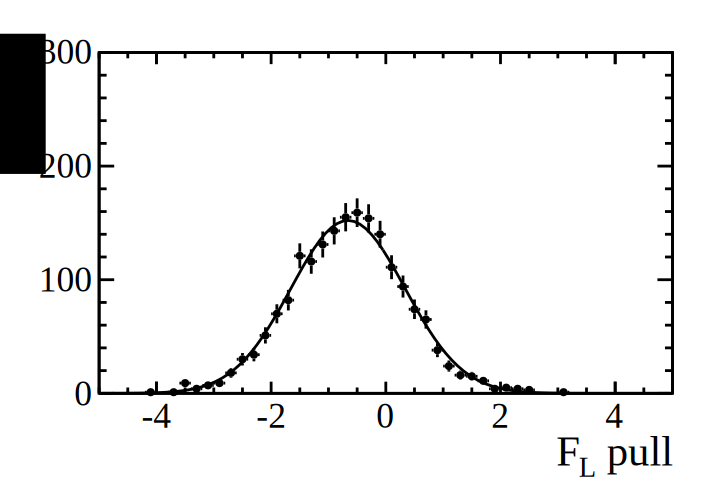
\includegraphics[width=0.48\textwidth]{chapter6/figs/fit_result_test_fl_gen_pull_plot_new.pdf}}
\caption[  Distribution of the results and pull  
values for \AFB (a,b) and \FL (c,d) respectively 
for fits to 1000 toy simulations each containing 1000 events. ]
{Distribution of the results and pull 
values for \AFB (a,b) and \FL (c,d) respectively 
for fits to 1000 toy simulations each containing 1000 events.
The S-wave is ignored in these fits. The resolution obtained on \AFB is 
$0.026\pm0.001$. Since the S-wave is ignored there is a non-zero 
pull mean for both observables at $(0.26\pm0.02)$ and $(-0.65\pm0.02)$ respectively. 
The widths of the pull distribution are consistent with unity at 
 $(1.01\pm0.01)$ and $(0.99\pm0.01)$.~\label{fig:toyexample}}
\end{figure}



\input{chapter6/analysis}

\section{Measuring the S-wave in \BdToKpill}
\label{sec:swave:measurement}

Obtaining unbiased values for the angular observables beyond the limits
 shown requires including the S-wave contribution in the angular model. % rather than ignoring it.
With the formalism developed in Section~\ref{sec:swave:theo}, three options are explored for measuring
it. The first option is to ignore the \psq dependence in the measured parameters and simply fit for
\psq-averaged values of \FS and \AS. The second option is to fit the \psq 
 line-shape simultaneously with the angular distribution.
This can be done in a small $p$ window between $800$ and $1000\mev$
or in the region from the lower kinematic threshold 
to $1200\mev$.
In all cases the datasets used to perform the 
studies are identical to those used in Sect. 5.1 
%The difference is in how the fit is performed.In each case, 
and the dataset and the S-wave sizes 
refer to the number of events in the smaller \psq window.

The angular distribution without \psq dependence is given in Eq.~\ref{eq:theo4dint}.
For each set of samples, the resolution and the mean 
and the width of the pull distribution of the angular observables are tested. 

The change in the resolution obtained on the angular observables 
for the three different methods of including the S-wave in the angular distribution
 (ignoring the \psq dependence, fitting a narrow \psq window and fitting a wide \psq window) 
is demonstrated by plotting the ratio with respect
to the resolution obtained when a single 
P-wave state is assumed.

The resolution and the mean of the pull distributions for the three different fit methods are shown
relative to the resolution and mean obtained using the assumption of a pure P-wave state. 
The ratio between the fit methods, including the S-wave in the angular distribution and 
assuming a P-wave state, as a function of dataset size
are shown in  Fig~\ref{fig:ratiods}.
\begin{figure}[tb]
\centering
\subfigure[\AFB]{\includegraphics[width=0.48\textwidth]{chapter6/figs/fit_result_ratio_ds_afb_res.pdf}}
\subfigure[\FL]{\includegraphics[width=0.48\textwidth]{chapter6/figs/fit_result_ratio_ds_fl_res.pdf}}
\subfigure[\AT2 ]{\includegraphics[width=0.48\textwidth]{chapter6/figs/fit_result_ratio_ds_at2_res.pdf}}
\subfigure[\AIm]{\includegraphics[width=0.48\textwidth]{chapter6/figs/fit_result_ratio_ds_aim_res.pdf}}
\caption[ Resolutions for three different methods to incorporate 
the S-wave relative to the resolution obtained when the S-wave is ignored.    ]
{Resolutions for three different methods to incorporate 
the S-wave relative to the resolution obtained when the S-wave is ignored. 
It can be seen that the best resolution is obtained when using the largest \psq window.
The original resolution is recovered to within 10\%. ~\label{fig:ratiods}}
\end{figure}
The pull mean for all three fit methods is shown in Fig~\ref{fig:combods}.
\begin{figure}[tb]
\centering
\subfigure[\AFB]{\includegraphics[width=0.48\textwidth]{chapter6/figs/fit_result_combo_ds_afb_mean.pdf}}
\subfigure[\FL]{\includegraphics[width=0.48\textwidth]{chapter6/figs/fit_result_combo_ds_fl_mean.pdf}}
\subfigure[\AT2 ]{\includegraphics[width=0.48\textwidth]{chapter6/figs/fit_result_combo_ds_at2_mean.pdf}}
\subfigure[\AIm]{\includegraphics[width=0.48\textwidth]{chapter6/figs/fit_result_combo_ds_aim_mean.pdf}}
\caption[ Pull mean for the three different  
methods to incorporate the S-wave and when the S-wave 
is ignored.      ]
{Pull mean for the three different  
methods to incorporate the S-wave and when the S-wave 
is ignored. There is a slight shift when the S-wave is 
included for datasets of less than 200 events but this is removed from  all the observables 
when the S-wave is included in the fit 
for datasets of over 500 events. ~\label{fig:combods}}
\end{figure}
The pull width for all three fit methods is shown in Fig~\ref{fig:combodswidth}.
\begin{figure}[tb]
\centering
\subfigure[\AFB]{\includegraphics[width=0.48\textwidth]{chapter6/figs/fit_result_combo_ds_afb_width.pdf}}
\subfigure[\FL]{\includegraphics[width=0.48\textwidth]{chapter6/figs/fit_result_combo_ds_fl_width.pdf}}
\subfigure[\AT2 ]{\includegraphics[width=0.48\textwidth]{chapter6/figs/fit_result_combo_ds_at2_width.pdf}}
\subfigure[\AIm]{\includegraphics[width=0.48\textwidth]{chapter6/figs/fit_result_combo_ds_aim_width.pdf}}
\caption[ Pull width for the three different  
methods to incorporate the S-wave and when the S-wave 
is ignored.  ]
{Pull width for the three different  
methods to incorporate the S-wave and when the S-wave 
is ignored. There is a slight shift when the S-wave is 
included for datasets of less than 200 events but this is removed from  all the observables 
when the S-wave is included in the fit 
for datasets of over 500 events. ~\label{fig:combodswidth}}
\end{figure}

For all observables, it can be seen that the resolution degrades when
the S-wave is included and the \psq dependence is ignored.  The
resolution degrades by a smaller amount when the \psq dependence is
included in a small bin and the original resolution is recovered to
within 10\% when using the large \psq range.  There are two effects
contributing to the improvement of the resolution. There are more
P-wave events in the larger range and the wider mass window allows for
the S-wave to be constrained by using the information from above and
below the P-wave resonance.  This results in the best resolution when
the S-wave is included in the angular distribution.

For all the observables, the pull mean approaches zero for datasets of
greater than 300 events implying that the bias present in the
observables when a pure P-wave state is assumed is removed when an S-wave is
included in the angular distribution. This means that the inclusion of
the S-wave component will be mandatory for all future experimental
analyses.


The ratio of the resolutions for the three different fit methods
as a function of increasing S-wave size is given in Fig.~\ref{fig:ratiofs}.
\begin{figure}[tb]
\centering
\subfigure[\AFB]{\includegraphics[width=0.48\textwidth]{chapter6/figs/fit_result_ratio_fs_afb_res.pdf}}
\subfigure[\FL]{\includegraphics[width=0.48\textwidth]{chapter6/figs/fit_result_ratio_fs_fl_res.pdf}}
\subfigure[\AT2 ]{\includegraphics[width=0.48\textwidth]{chapter6/figs/fit_result_ratio_fs_at2_res.pdf}}
\subfigure[\AIm]{\includegraphics[width=0.48\textwidth]{chapter6/figs/fit_result_ratio_fs_aim_res.pdf}}
\caption[  Resolutions for three different methods to incorporate 
the S-wave relative to the resolution obtained when the S-wave is ignored.   ]
{Resolutions for three different methods to incorporate 
the S-wave relative to the resolution obtained when the S-wave is ignored. 
It can be seen that the best resolution is obtained when using the largest \psq window.
The original resolution is recovered to within 10\%. ~\label{fig:ratiofs}}
\end{figure}
The pull mean  as a function of S-wave contribution 
for all three fit methods is shown in Fig.~\ref{fig:combofs}.
\begin{figure}[tb]
\centering
\subfigure[\AFB]{\includegraphics[width=0.48\textwidth]{chapter6/figs/fit_result_combo_fs_afb_mean.pdf}}
\subfigure[\FL]{\includegraphics[width=0.48\textwidth]{chapter6/figs/fit_result_combo_fs_fl_mean.pdf}}
\subfigure[\AT2 ]{\includegraphics[width=0.48\textwidth]{chapter6/figs/fit_result_combo_fs_at2_mean.pdf}}
\subfigure[\AIm]{\includegraphics[width=0.48\textwidth]{chapter6/figs/fit_result_combo_fs_aim_mean.pdf}}
\caption[ Pull mean for the three different  
methods to incorporate the S-wave and when the S-wave 
is ignored.    ]
{Pull mean for the three different  
methods to incorporate the S-wave and when the S-wave 
is ignored. There is a slight shift when the S-wave is 
included for datasets of less than 200 events but this is removed from  all the observables 
when the S-wave is included in the fit 
for datasets of over 500 events. ~\label{fig:combofs}}
\end{figure}
The pull width  as a function of S-wave contribution 
for all three fit methods is shown in Fig.~\ref{fig:combofswidth}.
\begin{figure}[tb]
\centering
\subfigure[\AFB]{\includegraphics[width=0.48\textwidth]{chapter6/figs/fit_result_combo_fs_afb_width.pdf}}
\subfigure[\FL]{\includegraphics[width=0.48\textwidth]{chapter6/figs/fit_result_combo_fs_fl_width.pdf}}
\subfigure[\AT2 ]{\includegraphics[width=0.48\textwidth]{chapter6/figs/fit_result_combo_fs_at2_width.pdf}}
\subfigure[\AIm]{\includegraphics[width=0.48\textwidth]{chapter6/figs/fit_result_combo_fs_aim_width.pdf}}
\caption[ Pull width for the three different  
methods to incorporate the S-wave and when the S-wave 
is ignored.    ]
{Pull width for the three different  
methods to incorporate the S-wave and when the S-wave 
is ignored. There is a slight shift when the S-wave is 
included for datasets of less than 200 events but this is removed from  all the observables 
when the S-wave is included in the fit 
for datasets of over 500 events. ~\label{fig:combofswidth}}
\end{figure}





\input{chapter6/isobar}

\section{Conclusions}

In summary, the inclusion of a resonant \kpi S-wave in the angular 
analysis of \BdToKstll  has been formalised and the complete angular 
distribution for both an S and P wave state described.
The inclusion of an S-wave state has an overall dilution
 effect on the theoretical observables.
The impact of an S-wave on an angular analysis is evaluated using toy 
Monte Carlo events.
The S-wave contribution can only be ignored for datasets of 
less than 200 events, meaning the angular observables measured in 
the \qsq bin between 4.3 and 8.68 \gevgevcccc and between
1 and 6 \gevgevcccc measured in Chapter 5 may be affected.
The bias on the angular observables incurred by assuming a pure P-wave
 \kpi state can be removed by including the S-wave in the angular distribution. 
The degradation in resolution on the angular observables 
from fitting a more complicated angular 
distribution can be minimised by performing the 
fit in a wide region around the $\Kstarz(892)$ resonance.
However, the parameterisation of the \mkpi spectrum also requires consideration 
of the background component in the wider \mkpi window which may increase the complexity
 and contribute other biases to measurements of the angular observables.




